\documentclass[11pt]{article}

\usepackage{amsmath,amssymb,amsthm}
\usepackage{hyperref}
\usepackage{enumitem}
\usepackage[utf8]{inputenc}
\usepackage{amsmath,amssymb,amsthm}
\usepackage{graphicx}
\usepackage{xcolor}

\usepackage{tikz}
\usepackage{pgfplots}
\pgfplotsset{compat=1.18}
\usetikzlibrary{3d}
\usetikzlibrary{3d,positioning}
\usepackage{tikz-3dplot}
\usepackage{tikz-cd}
\usepackage{caption}
\usepackage{subcaption}
\usepackage{geometry}
\geometry{margin=2cm}
\usetikzlibrary{arrows.meta,positioning,calc}
\usepackage{stmaryrd}

\title{Lecture Notes on Simplicial Homotopy Theory}
\author{Serkan Doğan}
\date{\today}

\theoremstyle{definition}
\newtheorem{definition}{Definition}[section]
\newtheorem{example}[definition]{Example}
\theoremstyle{plain}
\newtheorem{theorem}[definition]{Theorem}
\newtheorem{proposition}[definition]{Proposition}
\newtheorem{lemma}[definition]{Lemma}
\newtheorem{corollary}[definition]{Corollary}
\newtheorem{question}[definition]{Question}
\newtheorem{remark}[definition]{Remark}

\begin{document}

\maketitle

\tableofcontents

\section{Introduction}
This is the notes based on a weekly  seminar on simplicial homotopy theory. We mainly discussed simplicial objects in a category. I will give some motivation for the category of simplicial sets.

The origin of simplicial homotopy theory coincides with the beginning of algebraic topology. In algebraic topology, one studies homology and homotopy groups of topological spaces. We will recall some fundamental notions from algebraic topology.

\section{Fundamentals of Algebraic Topology}

The objects of algebraic topology are geometrically “nice” topological spaces, i.e., spaces that can be triangulated.

\subsection{Simplex }

The points of a finite set $P = \{p_0, p_1, \dots, p_k\} \subset \mathbb{R}^d$ are said to be \emph{affinely independent} if they are not contained in any affine subspace of dimension less than $k$. In other words, the set
\[
    \{p_1 - p_0, p_2 - p_0, \dots, p_k - p_0\}
\]
is a linearly independent set of vectors in $\mathbb{R}^d$.

\begin{definition}[Simplex]
    Given a set $P = \{p_0, p_1, \dots, p_k\} \subset \mathbb{R}^d$ of affinely independent points, the $k$-dimensional \emph{simplex} $\sigma$ (or $k$-simplex) spanned by $P$ is the set of convex combinations:
    \[
        \sum_{i=0}^{k} \lambda_i p_i, \quad \text{where } \lambda_i \geq 0, \ \sum_{i=0}^{k} \lambda_i = 1.
    \]
\end{definition}

The elements of $P$ are called the \emph{vertices} of the $k$-simplex $\sigma$.

\begin{example}
    \leavevmode
    \begin{itemize}
        \item A $0$-simplex is a point in $\mathbb{R}^d$.
        \item A $1$-simplex is a line segment between two points.
        \item A $2$-simplex is a filled-in triangle.
        \item A $3$-simplex is a filled-in tetrahedron.
    \end{itemize}
\end{example}

\begin{tikzpicture}

    % 1. şekil ve açıklaması
    \begin{scope}[xshift=0cm]
        \node (fig1) at (0,0) {
            \begin{tikzpicture}
                \begin{axis}[
                        width=5cm,
                        view={120}{30},
                        axis lines=middle,
                        ticks=none,
                        xmin=0, xmax=1.5,
                        ymin=0, ymax=1.5,
                        zmin=0, zmax=1.5,
                        xlabel={$x$}, ylabel={$y$}, zlabel={$z$}
                    ]
                    \addplot3[only marks, mark=*] coordinates {(0,1,0) (0,0,1)};
                    \addplot3[ultra thick] coordinates {(0,1,0) (0,0,1)};
                \end{axis}
            \end{tikzpicture}
        };
        \node[below=0.5cm of fig1, align=center] {A 1-simplex in $\mathbb{R}^3$ \\ with $P=\{(0,1,0),(0,0,1)\}$};
    \end{scope}

    % 2. şekil ve açıklaması (sadece x ekseni)
    \begin{scope}[xshift=6cm]
        \node (fig2) at (0,0) {
            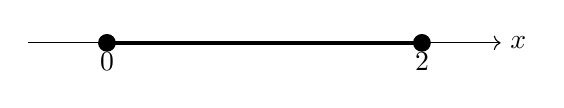
\begin{tikzpicture}[scale=2]
                % x-axis only
                \draw[->] (-0.5,0) -- (2.5,0) node[right] {$x$};
                \filldraw[black] (0,0) circle (1.5pt) node[below] {$0$};
                \filldraw[black] (2,0) circle (1.5pt) node[below] {$2$};
                \draw[ultra thick] (0,0) -- (2,0);
            \end{tikzpicture}
        };
        \node[below=0.5cm of fig2, align=center] {A 1-simplex in $\mathbb{R}$ \\ with $P=\{0,2\}$};
    \end{scope}

    % 3. şekil ve açıklaması
    \begin{scope}[xshift=12cm]
        \node (fig3) at (0,0) {
            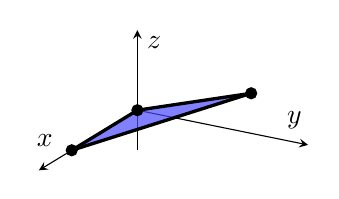
\begin{tikzpicture}
                \begin{axis}[
                        width=5cm,
                        view={120}{30},
                        axis lines=middle,
                        ticks=none,
                        xmin=0, xmax=3,
                        ymin=0, ymax=3,
                        zmin=-1, zmax=2,
                        xlabel={$x$}, ylabel={$y$}, zlabel={$z$}
                    ]
                    \addplot3[only marks, mark=*] coordinates {(0,0,0) (2,0,0) (0,2,1)};
                    \addplot3[fill=blue!70, opacity=0.7] coordinates {
                            (0,0,0)
                            (2,0,0)
                            (0,2,1)
                            (0,0,0)
                        };
                    \addplot3[very thick] coordinates {(0,0,0) (2,0,0)};
                    \addplot3[very thick] coordinates {(0,0,0) (0,2,1)};
                    \addplot3[very thick] coordinates {(2,0,0) (0,2,1)};
                \end{axis}
            \end{tikzpicture}
        };
        \node[below=0.5cm of fig3, align=center] {A 2-simplex in $\mathbb{R}^3$ \\ with $P=\{(0,0,0), (2,0,0), (0,2,1)\}$};
    \end{scope}

\end{tikzpicture}



The \emph{standard $n$-simplex} $\Delta^n$ is the subset of $\mathbb{R}^{n+1}$ given by
\[
    \Delta^n = \left\{ (t_0, t_1, \dots, t_n) \in \mathbb{R}^{n+1} \ \middle| \ t_i \geq 0,\ \sum_{i=0}^{n} t_i = 1 \right\}.
\]
The coordinates $t_i$ are called \emph{barycentric coordinates}. Here are

\begin{center}
    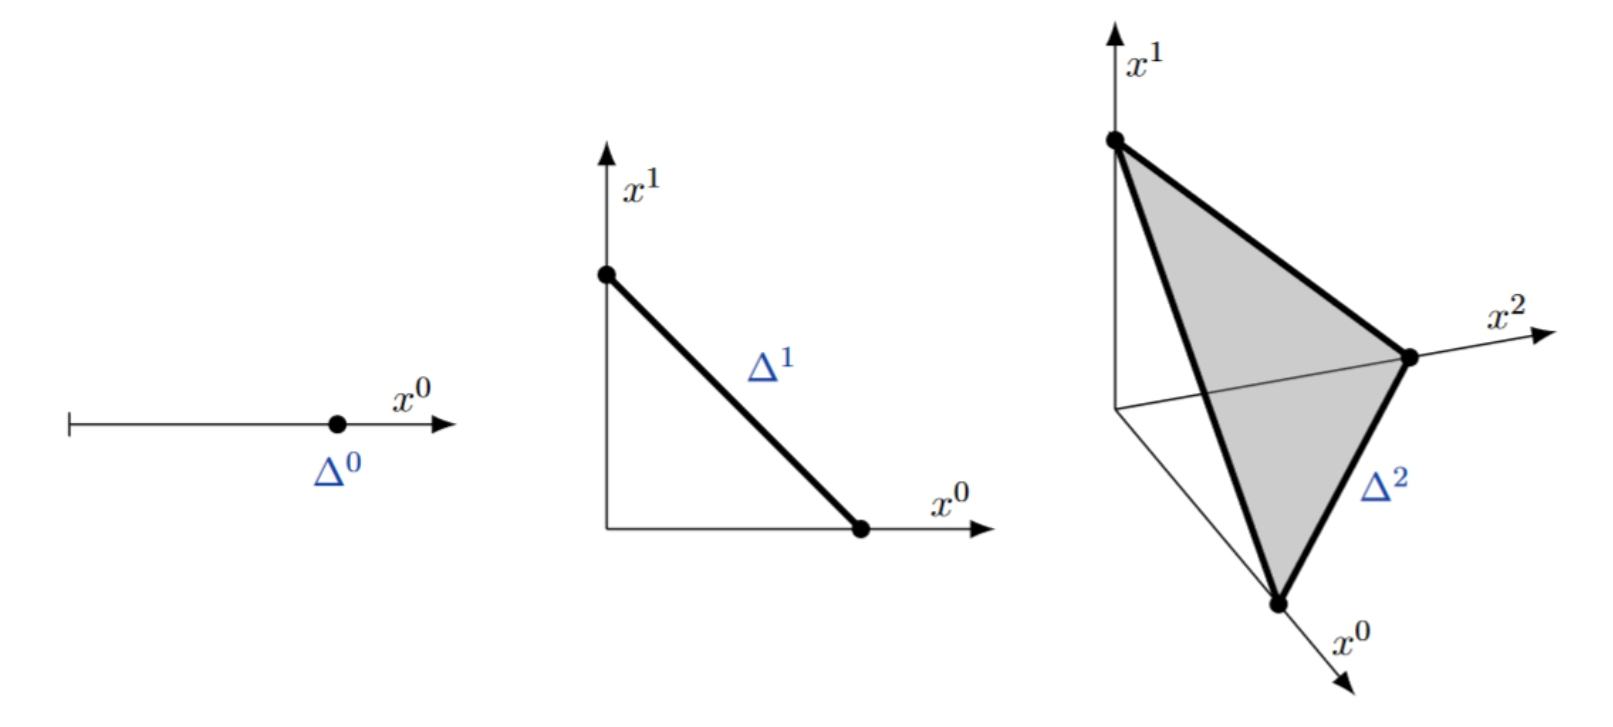
\includegraphics[height=5cm]{scp.jpg}
\end{center}

A face of a $k$-simplex $\sigma$ is the simplex spanned by a nonempty subset of the vertices of $\sigma$. In particular, the faces of a $k$-simplex include the simplex itself and its vertices.
As an example, a $2$-simplex has three $1$-dimensional faces (edges) and three $0$-dimensional faces (vertices).
\subsection{Geometric Simplicial Complexes}

A geometric simplicial complex is a collection of simplices that fit together in a nice way.



\begin{definition}[Simplicial Complex]
    A \emph{simplicial complex} $K$ in $\mathbb{R}^d$ is a collection of simplices satisfying the following conditions:
    \begin{enumerate}[label=(\roman*)]
        \item If $\sigma \in K$ is a simplex, then every face of $\sigma$ is also in $K$.
        \item If $\sigma, \tau \in K$, then their intersection is either empty or a face of both $\sigma$ and $\tau$.
    \end{enumerate}
\end{definition}

\textcolor{red}{Buraya bir tane örnek resim  koy.}



\begin{remark}
    For a simplicial complex $K$ in $\mathbb{R}^d$, its \emph{geometric realization} $|K| \subset \mathbb{R}^d$ is the union of the simplices of $K$. The topology on $|K|$ is the standard Euclidean topology.
\end{remark}

\begin{remark}
    A topological space $M$ is called \emph{triangulable} if it is homeomorphic to $|K|$ for some simplicial complex $K$. The space $|K|$ is then called a \emph{triangulation} of $M$. Not every topological space is triangulable, and a triangulation, when it exists, is not unique.
\end{remark}

As usual in mathematics we want to define structure-preserving maps between two objects. In this case , we say a map between two simplicial complexes is a simplicial map if it sends simplices to simplices in an affine way.

\begin{definition}[Simplicial Map between GSCs]
    Let $K$ and $L$ be geometric simplicial complexes. A map $f : K \to L$ is called a \emph{simplicial map} if:

    \begin{enumerate}
        \item For every simplex $\sigma \in K$, the image $f(\sigma)$ is contained in some simplex of $L$.
        \item The map $f$ is affine when restricted to each simplex of $K$.
    \end{enumerate}
\end{definition}

\begin{example}
    Let $K$ be a triangle with vertices $v_0, v_1, v_2$, and $L$ be a segment with vertices $w_0, w_1$.

    Define $f$ by:
    \[
        f(v_0) = w_0, \quad f(v_1) = w_1, \quad f(v_2) = w_1.
    \]

    Then $f$ is a simplicial map. Geometrically, we have:
    \begin{center}
        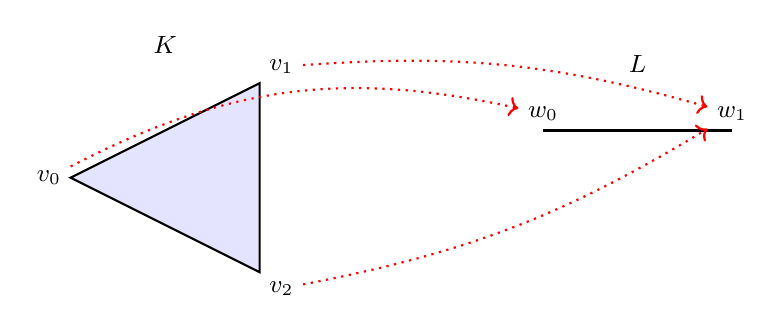
\begin{tikzpicture}[scale=1.2, every node/.style={font=\small}]
            % Triangle K (filled)
            \fill[blue!15, opacity=0.7] (0,0) -- (2,1) -- (2,-1) -- cycle;
            \draw[thick] (0,0) -- (2,1) -- (2,-1) -- cycle;
            \node[left] (v0) at (0,0) {$v_0$};
            \node[above right] (v1) at (2,1) {$v_1$};
            \node[below right] (v2) at (2,-1) {$v_2$};
            \node at (1, 1.4) {$K$};

            % Segment L
            \draw[thick] (5,0.5) -- (7,0.5);
            \node[above] (w0) at (5,0.5) {$w_0$};
            \node[above] (w1) at (7,0.5) {$w_1$};
            \node at (6, 1.2) {$L$};

            % Arrows from K to L
            \draw[->, thick, red, dotted] (v0) to[bend left=20] (w0);
            \draw[->, thick, red, dotted] (v1) to[bend left=10] (w1);
            \draw[->, thick, red, dotted] (v2) to[bend right=10] (w1);

        \end{tikzpicture}
    \end{center}

    The map $f$ is affine on each face and sends simplices in $K$ to simplices in $L$.
\end{example}

Geometric simplicial complexes are not combinatorial objects. However, we can encode the combinatorial data of a geometric simplicial complex in a purely combinatorial way. This leads us to the notion of abstract simplicial complexes.

\subsection{Abstract Simplicial Complexes}

To define a combinatorial version of a simplicial complex, we start with a finite set interpreted as vertices and consider certain subsets of it interpreted as faces.


\begin{definition}[Abstract Simplicial Complex]
    Let X be a finite set. An \emph{abstract simplicial complex} is a pair $(X, \Delta)$, where:
    \begin{itemize}
        \item $\Delta$ is a collection of nonempty subsets of $X$ (called \emph{simplices}) such that:

              If $\sigma \in \Delta$ and $\tau \subseteq \sigma$, then $\tau \in \Delta$.

    \end{itemize}
\end{definition}

\begin{example}
    Let $X = \{a, b, c, d\}$. Define a simplicial complex $\Delta$ by:
    \[
        \Delta = \{ \emptyset, \{a\}, \{b\}, \{c\}, \{d\}, \{a,b\}, \{a,c\}, \{b,c\}, \{a,b,c\} \}.
    \]
\end{example}
Geometrically, this can be visualized as a triangle with vertices $a, b, c$ and an isolated vertex $d$.
\begin{center}
    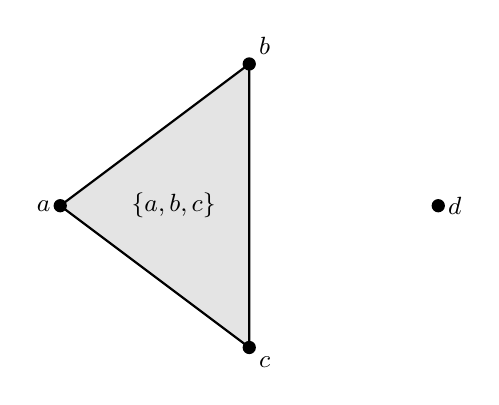
\begin{tikzpicture}[scale=1.2, every node/.style={font=\small}]
        % Triangle for a,b,c
        \coordinate (a) at (0,0);
        \coordinate (b) at (2,1.5);
        \coordinate (c) at (2,-1.5);
        \coordinate (d) at (4,0);

        % Draw triangle
        \fill[black!15, opacity=0.7] (a) -- (b) -- (c) -- cycle;
        \draw[thick] (a) -- (b) -- (c) -- (a);

        % Draw isolated vertex d
        \fill[black] (d) circle (2pt);
        \node[right] at (d) {$d$};

        % Draw vertices
        \fill[black] (a) circle (2pt);
        \fill[black] (b) circle (2pt);
        \fill[black] (c) circle (2pt);

        % Vertex labels
        \node[left] at (a) {$a$};
        \node[above right] at (b) {$b$};
        \node[below right] at (c) {$c$};

        % Edge labels (optional)
        %\node at ($(a)!0.5!(b)+(0,0.2)$) {$\{a,b\}$};
        %\node at ($(a)!0.5!(c)+(-0.1,-0.2)$) {$\{a,c\}$};
        %\node at ($(b)!0.5!(c)+(0.2,0)$) {$\{b,c\}$};

        % Triangle label
        \node at (1.2,0) {$\{a,b,c\}$};
    \end{tikzpicture}
\end{center}

\begin{example}[Non-example]
    Let $X = \{a, b, c\}$ and define
    \[
        \Delta' = \{ \{a\}, \{b\}, \{c\}, \{a,b\}, \{b,c\}, \{a,b,c\} \}.
    \]
    This is \emph{not} an abstract simplicial complex, because $\{a,c\}$ is a subset of $\{a,b,c\}$ but $\{a,c\} \notin \Delta'$. The definition requires that every nonempty subset of a simplex is also a simplex.
\end{example}

\paragraph{Terminology:}
\begin{itemize}
    \item Elements of $\Delta$ are called \emph{faces}.
    \item The \emph{dimension} of a face $\tau$ is $\#\tau - 1$.
    \item The \emph{dimension} of $\Delta$ is the maximum of the dimensions of its faces.
    \item $0$-dimensional faces are called \emph{vertices}.
    \item $1$-dimensional faces are called \emph{edges}.
    \item A simplicial complex of dimension at most $1$ is called a \emph{(multi-)graph}.
    \item A subcollection $\Delta' \subset \Delta$ that is itself a simplicial complex is called a \emph{subcomplex}.
    \item The \emph{$k$-skeleton} of $\Delta$ is the subcomplex consisting of all faces of dimension at most $k$.
\end{itemize}

Again , we want to define structure-preserving maps between two abstract simplicial complexes. In this case , we say a map between two abstract simplicial complexes is a simplicial map if it sends simplices to simplices.
More precisely:
\begin{definition}[Simplicial Map between ASCs]
    Let $(X, \Delta)$ and $(Y, \Gamma)$ be two abstract simplicial complexes.
    A \emph{simplicial map} $f : (X, \Delta) \to (Y, \Gamma)$ is a function $f : X \to Y$ such that for every simplex $\sigma \in \Delta$, the image $f(\sigma) := \{ f(v) \mid v \in \sigma \}$ belongs to $\Gamma$.
\end{definition}

\begin{example}
    Let:
    \[
        X = \{a, b, c\}, \quad \Delta = \{\{a\}, \{b\}, \{c\}, \{a,b\}, \{a,c\}\}
    \]
    \[
        Y = \{x, y\}, \quad \Gamma = \{\{x\}, \{y\}, \{x,y\}\}
    \]
    Define $f(a) = x$, $f(b) = y$, $f(c) = y$.

    Then $f$ is a simplicial map because the image of every simplex in $\Delta$ is a simplex in $\Gamma$.

    \begin{center}
        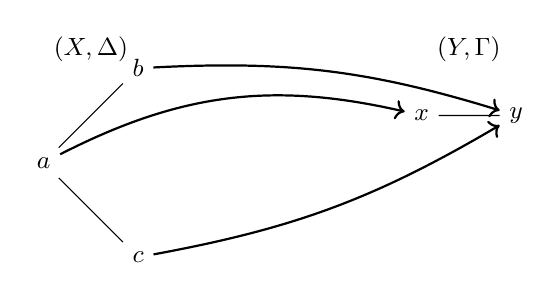
\begin{tikzpicture}[scale=1.2, every node/.style={font=\small}]
            % Domain complex
            \node (a) at (0,0) {$a$};
            \node (b) at (1,1) {$b$};
            \node (c) at (1,-1) {$c$};
            \draw (a) -- (b);
            \draw (a) -- (c);
            \node at (0.5, 1.2) {$(X, \Delta)$};

            % Codomain complex
            \node (x) at (4,0.5) {$x$};
            \node (y) at (5,0.5) {$y$};
            \draw (x) -- (y);
            \node at (4.5, 1.2) {$(Y, \Gamma)$};

            % Arrows
            \draw[->, thick] (a) to[bend left=20] (x);
            \draw[->, thick] (b) to[bend left=10] (y);
            \draw[->, thick] (c) to[bend right=10] (y);
        \end{tikzpicture}
    \end{center}

\end{example}






\subsection{Relation Between Geometric and Abstract Simplicial Complexes}

In this section, we define maps between abstract and geometric simplicial complexes and explore how abstract simplicial complexes can be realized geometrically.

\textbf{-From Abstract to Geometric: Geometric Realization}

Given an abstract simplicial complex $(X, \Delta)$, we can associate to it a topological space known as its \emph{geometric realization}, denoted $|\Delta|$.

\begin{definition}[Geometric Realization of an ASC]
    Let $(X, \Delta)$ be an abstract simplicial complex. The \emph{geometric realization} $|\Delta|$ is a topological space constructed as follows:
    \begin{itemize}
        \item Assign to each vertex $v \in X$ a point $e_v$ in some Euclidean space $\mathbb{R}^n$ such that the set $\{e_v \mid v \in X\}$ is affinely independent.
        \item For each simplex $\{v_0, \dots, v_k\} \in \Delta$, define the geometric $k$-simplex as:
              \[
                  \sigma = \left\{ \sum_{i=0}^{k} \lambda_i e_{v_i} \ \middle| \ \lambda_i \geq 0,\ \sum_{i=0}^{k} \lambda_i = 1 \right\}.
              \]
        \item The space $|\Delta|$ is the union of these geometric simplices, equipped with the subspace topology from $\mathbb{R}^n$.
    \end{itemize}
\end{definition}

\textbf{-From Geometric to Abstract}

Given a geometric simplicial complex $K$, we can form an abstract simplicial complex $(X, \Delta)$ by:
\begin{itemize}
    \item Letting $X$ be the set of vertices of $K$.
    \item Defining $\Delta$ to be the set of all finite subsets of $X$ that span simplices in $K$.
\end{itemize}

This correspondence defines a functorial relation between geometric and abstract simplicial complexes. However, note that geometric realizations are not unique — different embeddings can yield homeomorphic topological spaces.





\section{Singular Homology}

Singular homology is a fundamental tool in algebraic topology that assigns to each topological space a sequence of abelian groups (or modules), capturing information about its shape.


The standard simplices related by face inclusions:
\[
    d^i : \Delta^{n-1} \to \Delta^n \\
\]
\[
    d^i(t_0, \ldots, t_{n-1}) = (t_0, \ldots, t_{i-1}, 0, t_i, \ldots, t_{n-1}).
\]

For $0 \leq i \leq n $, the face map $d^i$ is the affine map that sends vertices to vertices in order and omits the  $i$-th vertex of the simplex $\Delta^n$.

\begin{center}
    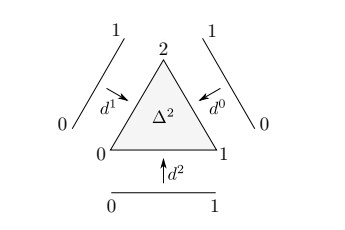
\includegraphics[height=5cm]{face_maps.jpg}
\end{center}


\begin{definition}[Singular $n$-Simplex]
    Let $X$ be a topological space.  A \emph{singular $n$-simplex} in a topological space $X$ is a continuous map $\sigma : \Delta^n \to X$, where $\Delta^n$ is the standard $n$-simplex.
    The set of all singular $n$-simplices in $X$ is denoted by $Sin_n(X)$.
\end{definition}
\begin{center}
    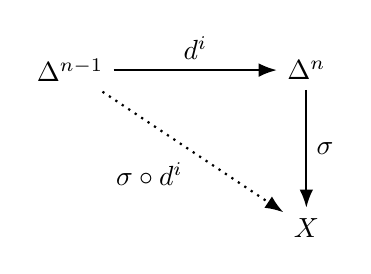
\begin{tikzpicture}[>=Latex, thick]

        % Nodes
        \node (A) at (0,2) {$\Delta^{n-1}$};
        \node (B) at (3,2) {$\Delta^n$};
        \node (C) at (3,0) {$X$};

        % Arrows
        \draw[->] (A) -- node[above] {$d^i$} (B);
        \draw[->] (B) -- node[right] {$\sigma$} (C);
        \draw[->, dotted] (A) -- node[below left] {$\sigma \circ d^i$} (C);

    \end{tikzpicture}
\end{center}

Therefore, the face map $d^i$ induce a map from the singular $n$-simplex $\sigma$ to the singular $(n-1)$-simplex $\sigma \circ d^i$. We have a map
\[
    d_i : Sin_n(X) \to Sin_{n-1}(X)
\]
\[
    d_i(\sigma)=\sigma \circ d^i
\]


\begin{definition}
    The Abelian group $S_n(X)$ of singular $n$-simplices in $X$ is defined as the free abelian group generated by all singular $n$-simplices in $X$. That is \[
        S_n(X)=\mathbb{Z}Sin_n(X)  \]
\end{definition}



For each $n \geq 1$, define the boundary operator $\partial_n : Sin_n(X) \to S_{n-1}(X)$ by
\[
    \partial_n(\sigma) = \sum_{i=0}^n (-1)^i d_i(\sigma) = \sum_{i=0}^n (-1)^i \sigma \circ d^i,
\]
where $d_i : \Delta^{n-1} \to \Delta^n$ is the $i$-th face map (inclusion of the $i$-th face).

This extends linearly to all of $S_n(X)$. One can check that $\partial_{n-1} \circ \partial_n = 0$ for all $n$, which is the most important property of the boundary operator.
This gives  a sequence of abelian groups and homomorphisms
\[
    \cdots \xrightarrow{\partial_{n+1}} S_n(X) \xrightarrow{\partial_n} S_{n-1}(X) \xrightarrow{\partial_{n-1}} \cdots \xrightarrow{\partial_1} S_0(X) \to 0.
\]
This sequence is called a \emph{ chain complex}  because $\partial_{n-1} \circ \partial_n = 0$ for all $n$. This property gives that  $\operatorname{im} \partial_{n+1} \subseteq \ker \partial_n$.

The $n$-th \emph{singular homology group} of $X$ is defined as

\[
    H_n(X) = \frac{\ker \partial_n}{\operatorname{im} \partial_{n+1}}.
\]

To define singular homology we used face maps between standard simplices. To define face maps we need to consider the standard simplices as oriented. These face maps can be seen as  order-preserving maps combinatorially. In fact, any order-preserving map between totally ordered sets induces an affine map between standard simplices.

\section{Ordered Simplicial Complexes}

An \emph{ordered simplicial complex} is an abstract simplicial complex equipped with a total ordering on its vertex set. This extra structure allows us to distinguish between different orderings of the same simplex, which is important in applications such as defining orientations or working with simplicial sets.

\begin{definition}[Ordered Simplicial Complex]
    An \emph{ordered simplicial complex} is a pair $(X, \Delta)$, where $X$ is a finite set with a total order, and $\Delta$ is a collection of nonempty subsets of $X$ such that:
    \begin{itemize}
        \item If $\sigma \in \Delta$ and $\tau \subseteq \sigma$, then $\tau \in \Delta$.
    \end{itemize}
    Each simplex $\sigma = \{v_0, v_1, \ldots, v_k\}$ is considered together with the induced order $v_0 < v_1 < \cdots < v_k$ from $X$.
\end{definition}

\begin{example}
    Let $X = \{a, b, c\}$ with $a < b < c$. Define
    \[
        \Delta = \{ \{a\}, \{b\}, \{c\}, \{a,b\}, \{b,c\}, \{a,c\}, \{a,b,c\} \}.
    \]
    Then $(X, \Delta)$ is an ordered simplicial complex. The $2$-simplex $\{a,b,c\}$ has the ordering $a < b < c$.
\end{example}


\begin{definition}[Simplicial Map between Ordered Simplicial  Complexes]
    Let $(X, \Delta)$ and $(Y, \Gamma)$ be ordered simplicial complexes, where $X$ and $Y$ are totally ordered sets. A \emph{simplicial map} $f : (X, \Delta) \to (Y, \Gamma)$ is a function $f : X \to Y$ such that:
    \begin{itemize}
        \item $f$ is order-preserving: if $v < w$ in $X$, then $f(v) < f(w)$ in $Y$,
        \item for every simplex $\sigma \in \Delta$, the image $f(\sigma) := \{ f(v) \mid v \in \sigma \}$ is a simplex in $\Gamma$.
    \end{itemize}
\end{definition}

\paragraph{Exercise.} Answer the following questions:
\begin{enumerate}[label=(\alph*)]
    \item Let $[n] $ denote the totally ordered set $\{0, 1, \ldots, n\}$. Let $\phi : [n] \to [m]$ be an order-preserving function(so that if $i \leq j$, then
          $\phi(i) \leq \phi(j)$). Identify the elements of $[n] $ with the vertices of
          the standard $n$-simplex $\Delta^n$. Show that $\phi$ induces an affine map $\Delta^n \to \Delta^m$. Give a formula for the induced map $\phi$
    \item Write $d^j : [n-1] \to [n] $ for the order-preserving map that skips the $j$-th element. Show that any order-preserving injection $\phi : [n-k] \to [n]$ can be written uniquely as a composition of the form $d^{j_k} \circ d^{j_{k-1}} \circ \cdots \circ d^{j_1}$ with $ 0 \leq j_1 < j_2 < \cdots < j_k \leq n$.
    \item Verify that $d^j \circ d^i = d^{i+1} \circ d^j$ if $i < j$.
    \item Show that any order-preserving map $\phi : [n] \to [m]$ can be written uniquely as a composition of an order-preserving injection $\phi' : [n-k] \to [m]$ followed by a surjective order-preserving map $\psi : [m] \to [m-k]$.
    \item Write $s^j : [n+1] \to [n]$ for the order-preserving map that repeats the $j$-th element. Show that any order-preserving surjection $\psi : [m] \to [n]$ can be written uniquely as a composition of the form $s^{j_k} \circ s^{j_{k-1}} \circ \cdots \circ s^{j_1}$ with $ 0 \leq j_1 < j_2 < \cdots < j_k \leq m$.
    \item Verify that $s^j \circ s^i = s^{i+1} \circ s^j$ if $i \leq j$.
    \item Find a formula for $s^i \circ d^j $
\end{enumerate}


\section{Category Theory Basics}

Category theory provides a unifying language for much of modern mathematics, including algebraic topology.
We will use category theoretical framework to translate classical homotopy theory to more combinatorial theory.
We recall some basic definitions and examples.

\subsection{Categories}

\begin{definition}[Category]
    A \emph{category} $\mathcal{C}$ consists of the following data:
    \begin{itemize}
        \item A class of \emph{objects} (denoted $A, B, C, \dots$).
        \item For each pair of objects $A, B$, a set of \emph{morphisms} (or \emph{arrows}) $\operatorname{Hom}_{\mathcal{C}}(A, B)$.
        \item For each triple $A, B, C$, a composition law: if $f \in \operatorname{Hom}_{\mathcal{C}}(A, B)$ and $g \in \operatorname{Hom}_{\mathcal{C}}(B, C)$, then $g \circ f \in \operatorname{Hom}_{\mathcal{C}}(A, C)$.
        \item For each object $A$, an \emph{identity morphism} $\mathrm{id}_A \in \operatorname{Hom}_{\mathcal{C}}(A, A)$.
    \end{itemize}
    These satisfy:
    \begin{itemize}
        \item \textbf{Associativity:} $(h \circ g) \circ f = h \circ (g \circ f)$ whenever the compositions make sense.
        \item \textbf{Identity:} For all $f \in \operatorname{Hom}_{\mathcal{C}}(A, B)$, $\mathrm{id}_B \circ f = f = f \circ \mathrm{id}_A$.
    \end{itemize}
\end{definition}


A category is a very general definition. The objects can be anything, and the morphisms can be any kind of structure-preserving maps. The key is that we have a way to compose morphisms and an identity morphism for each object.


\begin{itemize}
    \item [1]Categories as Structured Sets with Structure-Preserving Morphisms
          \begin{itemize}
              \item[(i)] \textbf{Set} Objects are sets, morphisms are functions between sets.
              \item[(ii)] \textbf{Top} Objects are topological spaces, morphisms are continuous maps.
              \item[(iii)] \textbf{Grp} Objects are groups, morphisms are group homomorphisms.
              \item[(iv)] \textbf{K-Vect} Objects are vector spaces over a field $k$, morphisms are linear maps.
              \item[(v)] \textbf{Rings:} Objects are rings (commutative or not, with or without identity, depending on context), morphisms are ring homomorphisms.
              \item[(vi)] \textbf{$R$-Mod} For a fixed ring $R$, objects are left $R$-modules, morphisms are $R$-linear maps.
              \item[(vii)] \textbf{Mnfld} Objects are smooth manifolds, morphisms are smooth maps.
              \item[(viii)] \textbf{Posets:} Any partially ordered set $(P, \leq)$ can be viewed as a category: objects are elements of $P$, and there is a unique morphism $x \to y$ if and only if $x \leq y$.
          \end{itemize}
    \item [2]Relations as Categories
          \begin{itemize}
              \item[(i)] \textbf{Equivalence Relations:} If $R$ is an equivalence relation on $X$, we can view $X$ as a category where:
                    \begin{itemize}
                        \item Objects are elements of $X$.
                        \item There is a unique morphism $x \to y$ if and only if $x \sim y$ (i.e., $x$ and $y$ are equivalent).

                    \end{itemize}
                    Each equivalence class forms a connected component (a groupoid with only identity morphisms between distinct objects in the same class).

                    \begin{example}
                        Consider $X = \{a, b, c\}$ with the equivalence relation $ \sim ={(a,a),(b,b),(c,c),(a,b),(b,a)} $. The associated category has:
                        \begin{itemize}
                            \item Objects: $a$, $b$, $c$.
                            \item Morphisms: For $x, y \in X$, a unique morphism $x \to y$ if $x \sim y$.
                        \end{itemize}
                        The morphisms are:
                        \begin{itemize}
                            \item $\mathrm{id}_a$, $\mathrm{id}_b$, $\mathrm{id}_c$ (identities)
                            \item $a \to b$, $b \to a$ (since $a \sim b$)
                        \end{itemize}

                        \begin{center}
                            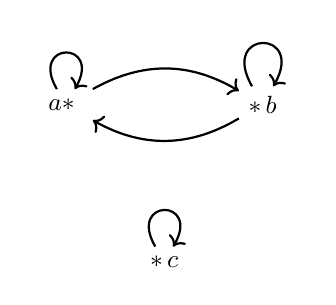
\begin{tikzpicture}[every node/.style={font=\small}, node distance=2.5cm]
                                \node (a) {$a \ast\ $};
                                \node (b) [right of=a] {$\ast\, b$};
                                \node (c) [below of=a, xshift=1.25cm, yshift=0.5cm] {$\ast\, c$};

                                \draw[->,thick] (a) to [out=120, in=60, looseness=8] (a);
                                \draw[->,thick] (b) to [out=120, in=60, looseness=8] (b);
                                \draw[->,thick] (c) to [out=120, in=60, looseness=8] (c);

                                \draw[->,thick,bend left=30] (a) to (b);
                                \draw[->,thick,bend left=30] (b) to (a);
                            \end{tikzpicture}
                        \end{center}


                    \end{example}


              \item[(ii)] \textbf{Posets:} If $R$ is a partial order $\leq$ on $X$, we get a category where:
                    \begin{itemize}
                        \item Objects are elements of $X$.
                        \item There is a unique morphism $x \to y$ if and only if $x \leq y$.

                    \end{itemize}
                    This is called the \emph{poset category} associated to $(X, \leq)$.

                    \begin{example}
                        Consider the poset $X = \{a, b, c\}$ with $a < b < c$. The associated category has:
                        \begin{itemize}
                            \item Objects: $a$, $b$, $c$.
                            \item Morphisms: There is a unique morphism $a \to b$, $b \to c$, and by composition $a \to c$. Each object has an identity morphism.
                        \end{itemize}
                        The diagram is:
                        \begin{center}
                            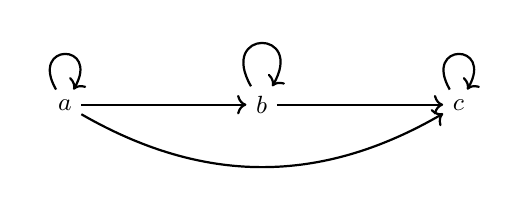
\begin{tikzpicture}[every node/.style={font=\small}, node distance=2.5cm]
                                \node (a) {$a$};
                                \node (b) [right of=a] {$b$};
                                \node (c) [right of=b] {$c$};

                                \draw[->,thick] (a) -- (b) node[midway,above] {};
                                \draw[->,thick] (b) -- (c) node[midway,above] {};
                                \draw[->,thick,bend right=30] (a) to (c);


                                \draw[->,thick,looseness=8,out=120,in=60] (a) to (a);
                                \draw[->,thick,looseness=8,out=120,in=60] (b) to (b);
                                \draw[->,thick,looseness=8,out=120,in=60] (c) to (c);
                            \end{tikzpicture}
                        \end{center}
                        Here, the morphisms are determined by the order: $a \to b$, $b \to c$, $a \to c$, and identities.
                    \end{example}
          \end{itemize}
    \item [3]operations as Categories
          \begin{itemize}
              \item[(i)] \textbf{Group as a Category :}
                    A group $G$ can be viewed as a category $BG$ with a single object $\ast$, where every morphism $\ast \to \ast$ is an element of $G$. Composition of morphisms is given by group multiplication, and the identity morphism is the identity element of $G$.
                    \begin{center}
                        \begin{tikzpicture}[scale=1.2, every node/.style={font=\small}]
                            % Tek nesne, sadece yıldız (dairenin olmaması için draw kaldırıldı)
                            \node (A) at (0,0) {$\ast$};

                            % Morfizmler için iç içe döngüler
                            \draw[->,thick,black,looseness=10,out=60,in=120] (A) to node[above] {0} (A);
                            \draw[->,thick,blue,looseness=20,out=30,in=150] (A) to node[above] {1} (A);
                            % id oku: açıları değiştirip daha geniş bir yay yaptık
                            \draw[->,thick,red,looseness=40,out=20,in=150] (A) to node[above] {2} (A);
                        \end{tikzpicture}
                    \end{center}

              \item[(ii)] \textbf{Monoid as a Category :}
                    Similarly, a monoid $M$ can be regarded as a category $BM$ with one object $\ast$, where morphisms $\ast \to \ast$ are elements of $M$, composition is monoid multiplication, and the identity morphism is the identity element of $M$.

          \end{itemize}


\end{itemize}





\subsection{Functors}

\begin{definition}[Functor]
    Let $\mathcal{C}$ and $\mathcal{D}$ be categories. A \emph{functor} $F : \mathcal{C} \to \mathcal{D}$ assigns:
    \begin{itemize}
        \item To each object $A$ of $\mathcal{C}$, an object $F(A)$ of $\mathcal{D}$.
        \item To each morphism $f : A \to B$ in $\mathcal{C}$, a morphism $F(f) : F(A) \to F(B)$ in $\mathcal{D}$,
    \end{itemize}
    such that:
    \begin{itemize}
        \item $F(\mathrm{id}_A) = \mathrm{id}_{F(A)}$ for all $A$.
        \item $F(g \circ f) = F(g) \circ F(f)$ for all composable $f, g$.
    \end{itemize}
\end{definition}


\begin{itemize}
    \item [1)]Categories as Structured Sets with Structure-Preserving Morphisms
          \begin{itemize}
              \item[(i)] \textbf{Forgetful Functor:} The forgetful functor $U : \mathbf{Grp} \to \mathbf{Set}$ sends a group to its underlying set and a group homomorphism to the underlying function.
              \item[(ii)] \textbf{Homology Functor:} For a fixed $n$, the $n$-th singular homology functor $H_n : \mathbf{Top} \to \mathbf{Ab}$ assigns to each topological space its $n$-th singular homology group, and to each continuous map the induced homomorphism on homology.
              \item[(iii)] \textbf{Free Abelian Group Functor:} The functor $F : \mathbf{Set} \to \mathbf{Ab}$ sends a set $X$ to the free abelian group generated by $X$, and a function $f : X \to Y$ to the group homomorphism extending $f$ linearly.
              \item[(iv)] \textbf{Vector Space with $X$ a Basis:} The functor $V : \mathbf{Set} \to \mathbf{Vect}_k$ sends a set $X$ to the vector space over $k$ with basis $X$, and a function $f : X \to Y$ to the linear map determined by $f$ on basis elements.
              \item[(v)] \textbf{Power Set Functor:} The functor $\mathcal{P} : \mathbf{Set} \to \mathbf{Set}$ sends a set $X$ to its power set $\mathcal{P}(X)$ and a function $f : X \to Y$ to the function $\mathcal{P}(f) : \mathcal{P}(X) \to \mathcal{P}(Y)$ given by $A \mapsto f(A)$.
          \end{itemize}
    \item [2)]Relations as Categories \\
          We leave the details of this case to the reader. A functor between two categories of relations corresponds to a function between the underlying sets that preserves the relation structure.
    \item [3)]Operations as Categories \\
          A functor between BG and BH corresponds to  a group homomorphism $f : G \to H$. A functor $F : BG \to Vect_K$ corresponds to a representation of the group $G$ on a vector space over a field $K$.



\end{itemize}


\subsection{Opposite Category}

\begin{definition}[Opposite Category]
    Given a category $\mathcal{C}$, the \emph{opposite category} $\mathcal{C}^{op}$ has the same objects as $\mathcal{C}$, but for $A, B$, $\operatorname{Hom}_{\mathcal{C}^{op}}(A, B) = \operatorname{Hom}_{\mathcal{C}}(B, A)$. Composition is defined by $(f : B \to A)$ followed by $(g : C \to B)$ is $f \circ g : C \to A$.
\end{definition}

\begin{example}
    A contravariant functor $F : \mathcal{C} \to \mathcal{D}$ is the same as a functor $F : \mathcal{C}^{op} \to \mathcal{D}$.
\end{example}

\subsection{Natural Transformations}

\begin{definition}[Natural Transformation]
    Let $F, G : \mathcal{C} \to \mathcal{D}$ be functors. A \emph{natural transformation} $\eta : F \Rightarrow G$ assigns to each object $A$ in $\mathcal{C}$ a morphism $\eta_A : F(A) \to G(A)$ in $\mathcal{D}$ such that for every morphism $f : A \to B$ in $\mathcal{C}$, the following diagram commutes:
    \[
        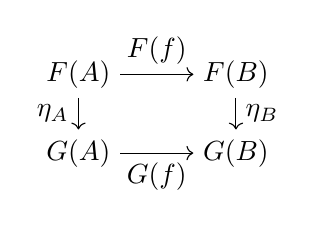
\begin{tikzpicture}[baseline=(current bounding box.center)]
            \node (FA) at (0,1) {$F(A)$};
            \node (FB) at (2,1) {$F(B)$};
            \node (GA) at (0,0) {$G(A)$};
            \node (GB) at (2,0) {$G(B)$};
            \draw[->] (FA) -- node[above] {$F(f)$} (FB);
            \draw[->] (GA) -- node[below] {$G(f)$} (GB);
            \draw[->] (FA) -- node[left] {$\eta_A$} (GA);
            \draw[->] (FB) -- node[right] {$\eta_B$} (GB);
        \end{tikzpicture}
    \]
    That is, $G(f) \circ \eta_A = \eta_B \circ F(f)$ for all $f$.
\end{definition}

\begin{example}
    Let $F, G : \mathbf{Set} \to \mathbf{Set}$ be functors, with $F(X) = X \times X$ and $G(X) = X$. The map $\eta_X : X \times X \to X$ given by $\eta_X(x, y) = x$ defines a natural transformation from $F$ to $G$.
\end{example}












\section{Simplicial Sets}
Let us look at the poset category in more detail.
We know that a partially ordered set $(X,\leq)$ is a category where the objects are the elements of X and there is a unique morphism from $x$ to $y$ if $x \leq y$.
Consider two posets $(X,\leq)$ and $(Y,\leq)$  What is a functor between them?
Let F be a funtor from X to Y.
Then F consists of the following data:
\begin{itemize}
    \item For each $x \in X$, an object $F(x) \in Y$. This just says that $F$ is a a function from $X$ to $Y$.
    \item For each $f \in Hom(x_1,x_2)$, a morphism $F(f) \in Hom(F(x_1),F(x_2))$.
          This means that if $x_1 \leq x_2$ in $X$, then $F(x_1) \leq F(x_2)$ in $Y$. In other words, $F$ is an order-preserving function.
\end{itemize}


Here is the main ingredient of the theory.
\begin{definition}[Simplex Category]
    The \emph{simplex category} $\Delta$ is the category whose objects are the finite ordered sets $[n] = \{0,1,\dots,n\}$ for $n \geq 0$, and whose morphisms are order-preserving (non-decreasing) functions between them.
\end{definition}

Each finite ordered set is isomorphic to the ordered set $[n]$ for some $n \geq 0$. Technically speaking, in $\Delta$, the objects are categories themselves, and the morphisms correspond to the functors between them.
On the other hand, to study the simplex category, we only need to consider the ordered set  $[n]$ and the set of non-decreasing functions between them.



\begin{example}

    All morphisms from $\mathbf{[2]}$ to $\mathbf{[1]}$.



    \begin{center}
        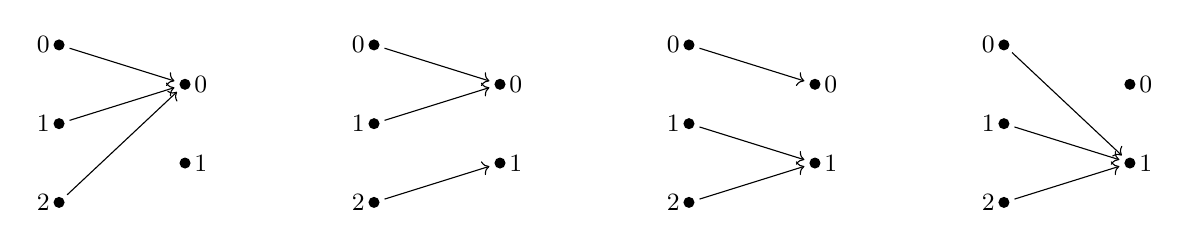
\begin{tikzpicture}[scale=1.0, font=\small]
            \tikzset{->, shorten >=4pt, shorten <=4pt}

            % First morphism
            \foreach \i/\y in {0/2, 1/1, 2/0} {
                    \node at (0,\y) {\i};
                    \fill (0.2,\y) circle (2pt); % domain dots
                }
            \foreach \i/\y in {0/1.5, 1/0.5} {
                    \node at (2,\y) {\i};
                    \fill (1.8,\y) circle (2pt); % codomain dots
                }
            \draw (0.2,2) -- (1.8,1.5);
            \draw (0.2,1) -- (1.8,1.5);
            \draw (0.2,0) -- (1.8,1.5);

            % Second morphism
            \begin{scope}[xshift=4cm]
                \foreach \i/\y in {0/2, 1/1, 2/0} {
                        \node at (0,\y) {\i};
                        \fill (0.2,\y) circle (2pt);
                    }
                \foreach \i/\y in {0/1.5, 1/0.5} {
                        \node at (2,\y) {\i};
                        \fill (1.8,\y) circle (2pt);
                    }
                \draw (0.2,2) -- (1.8,1.5);
                \draw (0.2,1) -- (1.8,1.5);
                \draw (0.2,0) -- (1.8,0.5);
            \end{scope}

            % Third morphism
            \begin{scope}[xshift=8cm]
                \foreach \i/\y in {0/2, 1/1, 2/0} {
                        \node at (0,\y) {\i};
                        \fill (0.2,\y) circle (2pt);
                    }
                \foreach \i/\y in {0/1.5, 1/0.5} {
                        \node at (2,\y) {\i};
                        \fill (1.8,\y) circle (2pt);
                    }
                \draw (0.2,2) -- (1.8,1.5);
                \draw (0.2,1) -- (1.8,0.5);
                \draw (0.2,0) -- (1.8,0.5);
            \end{scope}

            % Fourth morphism
            \begin{scope}[xshift=12cm]
                \foreach \i/\y in {0/2, 1/1, 2/0} {
                        \node at (0,\y) {\i};
                        \fill (0.2,\y) circle (2pt);
                    }
                \foreach \i/\y in {0/1.5, 1/0.5} {
                        \node at (2,\y) {\i};
                        \fill (1.8,\y) circle (2pt);
                    }
                \draw (0.2,2) -- (1.8,0.5);
                \draw (0.2,1) -- (1.8,0.5);
                \draw (0.2,0) -- (1.8,0.5);
            \end{scope}

        \end{tikzpicture}
    \end{center}

\end{example}


Here is another example.
\begin{example}
    All morphisms from $\mathbf{[1]}$ to $\mathbf{[2]}$

    \begin{center}
        \begin{tikzpicture}[scale=1.0, font=\small]
            \tikzset{->, shorten >=4pt, shorten <=4pt}

            % ---- FIRST ROW ----

            % (0,0)
            \foreach \i/\y in {0/1.5, 1/0.5} {
                    \node at (0,\y) {\i};
                    \fill (0.2,\y) circle (2pt);
                }
            \foreach \i/\y in {0/2, 1/1, 2/0} {
                    \node at (2,\y) {\i};
                    \fill (1.8,\y) circle (2pt);
                }
            \draw (0.2,1.5) -- (1.8,2);
            \draw (0.2,0.5) -- (1.8,2);

            % (0,1)
            \begin{scope}[xshift=4cm]
                \foreach \i/\y in {0/1.5, 1/0.5} {
                        \node at (0,\y) {\i};
                        \fill (0.2,\y) circle (2pt);
                    }
                \foreach \i/\y in {0/2, 1/1, 2/0} {
                        \node at (2,\y) {\i};
                        \fill (1.8,\y) circle (2pt);
                    }
                \draw (0.2,1.5) -- (1.8,2);
                \draw (0.2,0.5) -- (1.8,1);
            \end{scope}

            % (0,2)
            \begin{scope}[xshift=8cm]
                \foreach \i/\y in {0/1.5, 1/0.5} {
                        \node at (0,\y) {\i};
                        \fill (0.2,\y) circle (2pt);
                    }
                \foreach \i/\y in {0/2, 1/1, 2/0} {
                        \node at (2,\y) {\i};
                        \fill (1.8,\y) circle (2pt);
                    }
                \draw (0.2,1.5) -- (1.8,2);
                \draw (0.2,0.5) -- (1.8,0);
            \end{scope}

            % ---- SECOND ROW ----

            % (1,1)
            \begin{scope}[yshift=-4cm]
                \foreach \i/\y in {0/1.5, 1/0.5} {
                        \node at (0,\y) {\i};
                        \fill (0.2,\y) circle (2pt);
                    }
                \foreach \i/\y in {0/2, 1/1, 2/0} {
                        \node at (2,\y) {\i};
                        \fill (1.8,\y) circle (2pt);
                    }
                \draw (0.2,1.5) -- (1.8,1);
                \draw (0.2,0.5) -- (1.8,1);
            \end{scope}

            % (1,2)
            \begin{scope}[xshift=4cm, yshift=-4cm]
                \foreach \i/\y in {0/1.5, 1/0.5} {
                        \node at (0,\y) {\i};
                        \fill (0.2,\y) circle (2pt);
                    }
                \foreach \i/\y in {0/2, 1/1, 2/0} {
                        \node at (2,\y) {\i};
                        \fill (1.8,\y) circle (2pt);
                    }
                \draw (0.2,1.5) -- (1.8,1);
                \draw (0.2,0.5) -- (1.8,0);
            \end{scope}

            % (2,2)
            \begin{scope}[xshift=8cm, yshift=-4cm]
                \foreach \i/\y in {0/1.5, 1/0.5} {
                        \node at (0,\y) {\i};
                        \fill (0.2,\y) circle (2pt);
                    }
                \foreach \i/\y in {0/2, 1/1, 2/0} {
                        \node at (2,\y) {\i};
                        \fill (1.8,\y) circle (2pt);
                    }
                \draw (0.2,1.5) -- (1.8,0);
                \draw (0.2,0.5) -- (1.8,0);
            \end{scope}

        \end{tikzpicture}
    \end{center}

\end{example}

\begin{remark}
    The morphisms in the simplex category $\Delta$ are not necessarily injective. There is also a category of finite ordered sets, with injective order-preserving maps as morphisms.
\end{remark}

\begin{definition}[Delta Category ]
    The \emph{category} $\Delta_{inj} $ is the category whose objects are the finite ordered sets $[n] = \{0,1,\dots,n\}$ for each $n \geq 0$, and whose morphisms are all injective order-preserving  functions between them. That is, a morphism $\phi : [n] \to [m]$ satisfies $\phi(i) < \phi(j)$ whenever $i < j$.
\end{definition}
Note that if $ m<n$ then $Hom_{\Delta_{inj}}([n],[m]) = \emptyset$.
Thus, we do not have morphisms from $[2]$ to $[1]$. However we do have morphisms from $[1]$ to $[2]$ in $\Delta_{inj}$. As an example , look at the example 6.3 , 3 of the morphisms are injective.

We will not use the category $\Delta_{inj}$ in this course, but it is worth noting that it is a subcategory of the simplex category $\Delta$.



There are special morphisms in the simplex category $\Delta$ that is a generating set for the morphisms in $\Delta$.

\begin{definition}[co-Face and co-Degeneracy Maps]
    For each $n \geq 0$, the simplex category $\Delta$ has special morphisms:
    \begin{itemize}
        \item The $i$-th \emph{co-face map} $d^i : [n-1] \to [n]$ is the injective order-preserving map that skips $i$. Here is the formula for the $i$-th co-face map:
              \begin{align*}
                  d^i : [n-1] & \to [n] \\
                  d^i(x)      & =
                  \begin{cases}
                      x     & \text{if } x < i    \\
                      x + 1 & \text{if } x \geq i
                  \end{cases}
              \end{align*}

        \item The $i$-th \emph{co-degeneracy map} $s^i : [n+1] \to [n]$ is the surjective order-preserving map that repeats $i$. Here is the formula for the $i$-th co-degeneracy map:

              \begin{align*}
                  s^i : [n+1] & \to [n] \\
                  s^i(x)      & =
                  \begin{cases}
                      x     & \text{if } x \leq i \\
                      x - 1 & \text{if } x > i
                  \end{cases}
              \end{align*}

    \end{itemize}


\end{definition}
Any morphism in the simplex category $\Delta$ can be expressed as a composition of a surjection followed by an injection. In the exercise at the end of the 4th chapter, we asked you to verify any injection order-preserving map can be expressed as a composition of the co-face maps.
Similarly, any surjection order-preserving map can be expressed as a composition of the co-degeneracy maps. Therefore, co-face and co-degeneracy maps generate the morphisms in the simplex category $\Delta$.
However , they are not free generators, they satisfy some identities.

\begin{proposition}[Cosimplicial Identities]
    The co-face and co-degeneracy maps in the simplex category $\Delta$ satisfy the following \emph{cosimplicial identities} for all $i, j$:
    \begin{align*}
        d^j d^i & = d^i d^{j-1} \quad \text{if } i < j      \\
        s^j s^i & = s^{i} s^{j+1} \quad \text{if } i \leq j \\
        s^j d^i & =
        \begin{cases}
            d^i s^{j-1} & \text{if } i < j                     \\
            \mathrm{id} & \text{if } i = j \text{ or } i = j+1 \\
            d^{i-1} s^j & \text{if } i > j+1
        \end{cases}
    \end{align*}
\end{proposition}


Now, we are ready to define simplicial sets.
\begin{definition}
    A \emph{simplicial set} is a functor $X: \Delta^{op} \to \mathbf{Set}$, where $\Delta$ is the simplex category.
\end{definition}

Let us elaborate this definition. for each $n \geq 0$, the simplicial set $X$ assigns a set $X_n = X([n])$.
for each morphism $f: [m] \to [n]$ in $\Delta^{op}$, we have a map $X(f): X_n \to X_m$.
We know that each morphisms in $\Delta$ is a composition of co-face and co-degeneracy maps. Let us denote the face maps by $d_i=(d^i)^*$ and the degeneracy maps by $s_i=(s^i)^*$. Then, we have the following maps for each $n \geq 0$:
\[
    d_i : X_n \to X_{n-1} \quad (0 \leq i \leq n), \qquad s_i : X_n \to X_{n+1} \quad (0 \leq i \leq n)
\]
satisfying the \emph{simplicial identities}:
\begin{align*}
    d_i d_j & = d_{j-1} d_i \quad \text{if } i < j    \\
    s_i s_j & = s_{j+1} s_i \quad \text{if } i \leq j \\
    d_i s_j & =
    \begin{cases}
        s_{j-1} d_i & \text{if } i < j                     \\
        \mathrm{id} & \text{if } i = j \text{ or } i = j+1 \\
        s_j d_{i-1} & \text{if } i > j+1
    \end{cases}
\end{align*}

These maps are called the \emph{face maps} and \emph{degeneracy maps} of the simplicial set $X$.
\begin{example}
    Let $X$ be a set and let $K_n =\prod_{i=0}^n X=X^{n+1}$ be the set of $(n+1)$-tuples of elements in $X$. Then, we can define a simplicial set $K$ as follows:
    \begin{itemize}
        \item For each $n \geq 0$, let $K_n = X^{n+1}$.
        \item The face maps $d_i : K_n \to K_{n-1}$ are defined by forgetting the $i$-th element of the tuple.
              \begin{align*}
                  d_i(x_0, x_1, \ldots, x_n) & = (x_0, \ldots, x_{i-1}, x_{i+1}, \ldots, x_n) \quad (0 \leq i \leq n)
              \end{align*}
        \item The degeneracy maps $s_i : K_n \to K_{n+1}$ are defined by repeating the $i$-th element of the tuple.
              \begin{align*}
                  s_i(x_0, x_1, \ldots, x_n) & = (x_0, \ldots, x_i, x_i, x_{i+1}, \ldots, x_n) \quad (0 \leq i \leq n)
              \end{align*}
    \end{itemize}

\end{example}


\begin{example}
    The \emph{nerve} of a category $\mathcal{C}$ is a simplicial set defined as follows:
    \begin{itemize}
        \item For each $n \geq 0$, let $N(\mathcal{C})_n$ be the set of $(n+1)$-tuples of composable morphisms in $\mathcal{C}$.
              \[
                  N(\mathcal{C})_n = \left\{
                  \begin{tikzcd}[column sep=2.5em,ampersand replacement=\&]
                      C_0 \arrow[r, "f_1"] \& C_1 \arrow[r, "f_2"] \& \cdots \arrow[r, "f_n"] \& C_n
                  \end{tikzcd}
                  \ \middle| \
                  f_i : C_{i-1} \to C_i \text{ in } \mathcal{C}
                  \right\}
              \]
        \item The face maps $d_i : N(\mathcal{C})_n \to N(\mathcal{C})_{n-1}$ compose the $i$-th and $(i+1)$-st morphisms in the sequence. That is, for a sequence of composable morphisms
              \[
                  \begin{tikzcd}[column sep=2.5em,ampersand replacement=\&]
                      C_0 \arrow[r, "f_1"] \& C_1 \arrow[r, "f_2"] \& \cdots \arrow[r, "f_n"] \& C_n
                  \end{tikzcd}
              \]
              the $i$-th face map ($0 \leq i \leq n$) is given by
              \[
                  d_i(f_1, \ldots, f_n) =
                  \begin{cases}
                      (f_2, \ldots, f_n)                            & i = 0             \\
                      (f_1, \ldots, f_i \circ f_{i+1}, \ldots, f_n) & 1 \leq i \leq n-1 \\
                      (f_1, \ldots, f_{n-1})                        & i = n
                  \end{cases}
              \]
        \item The degeneracy maps $s_i : N(\mathcal{C})_n \to N(\mathcal{C})_{n+1}$ insert an identity morphism at position $i$. That is, for
              \[
                  \begin{tikzcd}[column sep=2.5em,ampersand replacement=\&]
                      C_0 \arrow[r, "f_1"] \& C_1 \arrow[r, "f_2"] \& \cdots \arrow[r, "f_n"] \& C_n
                  \end{tikzcd}
              \]
              the $i$-th degeneracy map ($0 \leq i \leq n$) is
              \[
                  s_i(f_1, \ldots, f_n) = (f_1, \ldots, f_i, \mathrm{id}_{C_i}, f_{i+1}, \ldots, f_n)
              \]
              which corresponds to the diagram
              \[
                  \begin{tikzcd}[column sep=2.5em,ampersand replacement=\&]
                      C_0 \arrow[r, "f_1"] \& \cdots \arrow[r, "f_i"] \& C_i \arrow[r, "\mathrm{id}_{C_i}"] \& C_i \arrow[r, "f_{i+1}"] \& \cdots \arrow[r, "f_n"] \& C_n
                  \end{tikzcd}
              \]

    \end{itemize}

\end{example}


\begin{example}[Nerve of a Group]
    Let $G$ be a group, and consider the category $BG$ with a single object $\ast$ and morphisms $\operatorname{Hom}(\ast, \ast) = G$. The nerve $N_\bullet(BG)$ is a simplicial set where:
    \begin{itemize}
        \item $N(BG)_n = G^n$ for $n \geq 0$ (by convention, $G^0$ is a singleton).
        \item The face maps $d_i : G^n \to G^{n-1}$ are given by:
              \[
                  d_i(g_1, \ldots, g_n) =
                  \begin{cases}
                      (g_2, \ldots, g_n)                      & i = 0             \\
                      (g_1, \ldots, g_i g_{i+1}, \ldots, g_n) & 1 \leq i \leq n-1 \\
                      (g_1, \ldots, g_{n-1})                  & i = n
                  \end{cases}
              \]
        \item The degeneracy maps $s_j : G^n \to G^{n+1}$ are given by:
              \[
                  s_j(g_1, \ldots, g_n) = (g_1, \ldots, g_j, e, g_{j+1}, \ldots, g_n)
              \]
              where $e$ is the identity element of $G$.
    \end{itemize}
\end{example}


To form a category of simplicial sets, we need to define morphisms between them.


\begin{definition}[Simplicial Map]
    Let $X, Y : \Delta^{op} \to \mathbf{Set}$ be simplicial sets. A \emph{simplicial map} $f : X \to Y$ is a natural transformation of functors; that is, for each $n \geq 0$, a function $f_n : X_n \to Y_n$ such that for every morphism $\phi : [m] \to [n]$ in $\Delta$, the following diagram commutes:
    \[
        \begin{tikzcd}
            X_n \arrow[r,"f_n"] \arrow[d,"X(\phi^*)"'] & Y_n \arrow[d,"Y(\phi^*)"] \\
            X_m \arrow[r,"f_m"'] & Y_m
        \end{tikzcd}
    \]

\end{definition}

Let's elaborate the definition. A simplicial map $f : X \to Y$ between simplicial sets consists of a sequence of functions $f_n : X_n \to Y_n$ for each $n \geq 0$, compatible with the face and degeneracy maps. That is, for all $n \geq 0$ and $0 \leq i \leq n$, the following diagrams commute:
\[
    \begin{tikzcd}
        X_n \arrow[r,"f_n"] \arrow[d,"d_i"'] & Y_n \arrow[d,"d_i"] \\
        X_{n-1} \arrow[r,"f_{n-1}"'] & Y_{n-1}
    \end{tikzcd}
    \qquad
    \begin{tikzcd}
        X_n \arrow[r,"f_n"] \arrow[d,"s_i"'] & Y_n \arrow[d,"s_i"] \\
        X_{n+1} \arrow[r,"f_{n+1}"'] & Y_{n+1}
    \end{tikzcd}
\]
In other words, $f$ preserves the simplicial structure: it sends $n$-simplices to $n$-simplices in a way that is compatible with taking faces and degeneracies. This is analogous to how a continuous map between topological spaces preserves the structure of open sets, or how a group homomorphism preserves the group operation.
















\section{Simplicial homotopy and Kan complexes}










\section{References}
\begin{itemize}
    \item Goerss, P. G., \& Jardine, J. F. (2009). \emph{Simplicial Homotopy Theory}.
    \item May, J. P. (1992). \emph{Simplicial Objects in Algebraic Topology}.
\end{itemize}

\end{document}